% Created by tikzDevice version 0.12 on 2019-04-02 22:26:44
% !TEX encoding = UTF-8 Unicode
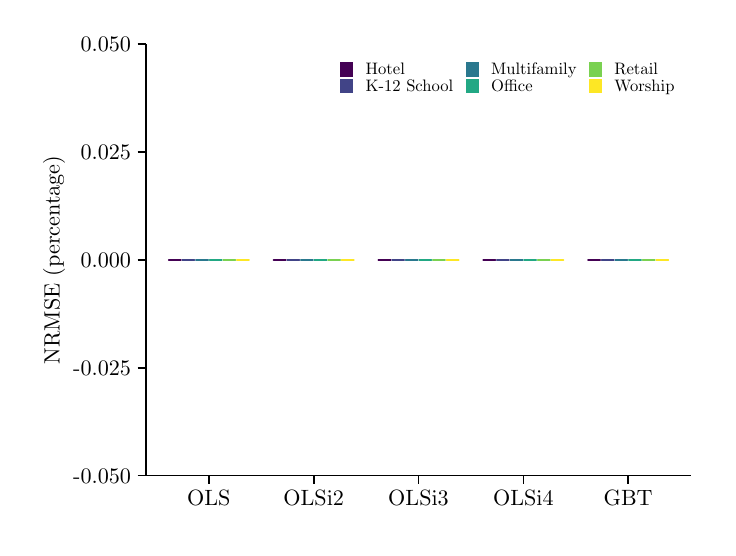
\begin{tikzpicture}[x=1pt,y=1pt]
\definecolor{fillColor}{RGB}{255,255,255}
\path[use as bounding box,fill=fillColor,fill opacity=0.00] (0,0) rectangle (245.72,180.67);
\begin{scope}
\path[clip] (  0.00,  0.00) rectangle (245.72,180.67);
\definecolor{drawColor}{RGB}{255,255,255}
\definecolor{fillColor}{RGB}{255,255,255}

\path[draw=drawColor,line width= 0.6pt,line join=round,line cap=round,fill=fillColor] (  0.00,  0.00) rectangle (245.72,180.68);
\end{scope}
\begin{scope}
\path[clip] ( 42.74, 18.85) rectangle (239.72,174.67);
\definecolor{fillColor}{RGB}{255,255,255}

\path[fill=fillColor] ( 42.74, 18.85) rectangle (239.72,174.67);
\definecolor{drawColor}{RGB}{253,231,37}
\definecolor{fillColor}{RGB}{253,231,37}

\path[draw=drawColor,line width= 0.6pt,line join=round,fill=fillColor] ( 75.57, 96.76) rectangle ( 79.99, 96.76);
\definecolor{drawColor}{RGB}{122,209,81}
\definecolor{fillColor}{RGB}{122,209,81}

\path[draw=drawColor,line width= 0.6pt,line join=round,fill=fillColor] ( 70.64, 96.76) rectangle ( 75.06, 96.76);
\definecolor{drawColor}{RGB}{34,168,132}
\definecolor{fillColor}{RGB}{34,168,132}

\path[draw=drawColor,line width= 0.6pt,line join=round,fill=fillColor] ( 65.72, 96.76) rectangle ( 70.14, 96.76);
\definecolor{drawColor}{RGB}{42,120,142}
\definecolor{fillColor}{RGB}{42,120,142}

\path[draw=drawColor,line width= 0.6pt,line join=round,fill=fillColor] ( 60.79, 96.76) rectangle ( 65.21, 96.76);
\definecolor{drawColor}{RGB}{65,68,135}
\definecolor{fillColor}{RGB}{65,68,135}

\path[draw=drawColor,line width= 0.6pt,line join=round,fill=fillColor] ( 55.87, 96.76) rectangle ( 60.29, 96.76);
\definecolor{drawColor}{RGB}{68,1,84}
\definecolor{fillColor}{RGB}{68,1,84}

\path[draw=drawColor,line width= 0.6pt,line join=round,fill=fillColor] ( 50.95, 96.76) rectangle ( 55.36, 96.76);
\definecolor{drawColor}{RGB}{253,231,37}
\definecolor{fillColor}{RGB}{253,231,37}

\path[draw=drawColor,line width= 0.6pt,line join=round,fill=fillColor] (113.45, 96.76) rectangle (117.87, 96.76);
\definecolor{drawColor}{RGB}{122,209,81}
\definecolor{fillColor}{RGB}{122,209,81}

\path[draw=drawColor,line width= 0.6pt,line join=round,fill=fillColor] (108.52, 96.76) rectangle (112.94, 96.76);
\definecolor{drawColor}{RGB}{34,168,132}
\definecolor{fillColor}{RGB}{34,168,132}

\path[draw=drawColor,line width= 0.6pt,line join=round,fill=fillColor] (103.60, 96.76) rectangle (108.02, 96.76);
\definecolor{drawColor}{RGB}{42,120,142}
\definecolor{fillColor}{RGB}{42,120,142}

\path[draw=drawColor,line width= 0.6pt,line join=round,fill=fillColor] ( 98.67, 96.76) rectangle (103.09, 96.76);
\definecolor{drawColor}{RGB}{65,68,135}
\definecolor{fillColor}{RGB}{65,68,135}

\path[draw=drawColor,line width= 0.6pt,line join=round,fill=fillColor] ( 93.75, 96.76) rectangle ( 98.17, 96.76);
\definecolor{drawColor}{RGB}{68,1,84}
\definecolor{fillColor}{RGB}{68,1,84}

\path[draw=drawColor,line width= 0.6pt,line join=round,fill=fillColor] ( 88.83, 96.76) rectangle ( 93.25, 96.76);
\definecolor{drawColor}{RGB}{253,231,37}
\definecolor{fillColor}{RGB}{253,231,37}

\path[draw=drawColor,line width= 0.6pt,line join=round,fill=fillColor] (151.33, 96.76) rectangle (155.75, 96.76);
\definecolor{drawColor}{RGB}{122,209,81}
\definecolor{fillColor}{RGB}{122,209,81}

\path[draw=drawColor,line width= 0.6pt,line join=round,fill=fillColor] (146.40, 96.76) rectangle (150.82, 96.76);
\definecolor{drawColor}{RGB}{34,168,132}
\definecolor{fillColor}{RGB}{34,168,132}

\path[draw=drawColor,line width= 0.6pt,line join=round,fill=fillColor] (141.48, 96.76) rectangle (145.90, 96.76);
\definecolor{drawColor}{RGB}{42,120,142}
\definecolor{fillColor}{RGB}{42,120,142}

\path[draw=drawColor,line width= 0.6pt,line join=round,fill=fillColor] (136.56, 96.76) rectangle (140.98, 96.76);
\definecolor{drawColor}{RGB}{65,68,135}
\definecolor{fillColor}{RGB}{65,68,135}

\path[draw=drawColor,line width= 0.6pt,line join=round,fill=fillColor] (131.63, 96.76) rectangle (136.05, 96.76);
\definecolor{drawColor}{RGB}{68,1,84}
\definecolor{fillColor}{RGB}{68,1,84}

\path[draw=drawColor,line width= 0.6pt,line join=round,fill=fillColor] (126.71, 96.76) rectangle (131.13, 96.76);
\definecolor{drawColor}{RGB}{253,231,37}
\definecolor{fillColor}{RGB}{253,231,37}

\path[draw=drawColor,line width= 0.6pt,line join=round,fill=fillColor] (189.21, 96.76) rectangle (193.63, 96.76);
\definecolor{drawColor}{RGB}{122,209,81}
\definecolor{fillColor}{RGB}{122,209,81}

\path[draw=drawColor,line width= 0.6pt,line join=round,fill=fillColor] (184.29, 96.76) rectangle (188.71, 96.76);
\definecolor{drawColor}{RGB}{34,168,132}
\definecolor{fillColor}{RGB}{34,168,132}

\path[draw=drawColor,line width= 0.6pt,line join=round,fill=fillColor] (179.36, 96.76) rectangle (183.78, 96.76);
\definecolor{drawColor}{RGB}{42,120,142}
\definecolor{fillColor}{RGB}{42,120,142}

\path[draw=drawColor,line width= 0.6pt,line join=round,fill=fillColor] (174.44, 96.76) rectangle (178.86, 96.76);
\definecolor{drawColor}{RGB}{65,68,135}
\definecolor{fillColor}{RGB}{65,68,135}

\path[draw=drawColor,line width= 0.6pt,line join=round,fill=fillColor] (169.51, 96.76) rectangle (173.93, 96.76);
\definecolor{drawColor}{RGB}{68,1,84}
\definecolor{fillColor}{RGB}{68,1,84}

\path[draw=drawColor,line width= 0.6pt,line join=round,fill=fillColor] (164.59, 96.76) rectangle (169.01, 96.76);
\definecolor{drawColor}{RGB}{253,231,37}
\definecolor{fillColor}{RGB}{253,231,37}

\path[draw=drawColor,line width= 0.6pt,line join=round,fill=fillColor] (227.09, 96.76) rectangle (231.51, 96.76);
\definecolor{drawColor}{RGB}{122,209,81}
\definecolor{fillColor}{RGB}{122,209,81}

\path[draw=drawColor,line width= 0.6pt,line join=round,fill=fillColor] (222.17, 96.76) rectangle (226.59, 96.76);
\definecolor{drawColor}{RGB}{34,168,132}
\definecolor{fillColor}{RGB}{34,168,132}

\path[draw=drawColor,line width= 0.6pt,line join=round,fill=fillColor] (217.24, 96.76) rectangle (221.66, 96.76);
\definecolor{drawColor}{RGB}{42,120,142}
\definecolor{fillColor}{RGB}{42,120,142}

\path[draw=drawColor,line width= 0.6pt,line join=round,fill=fillColor] (212.32, 96.76) rectangle (216.74, 96.76);
\definecolor{drawColor}{RGB}{65,68,135}
\definecolor{fillColor}{RGB}{65,68,135}

\path[draw=drawColor,line width= 0.6pt,line join=round,fill=fillColor] (207.39, 96.76) rectangle (211.81, 96.76);
\definecolor{drawColor}{RGB}{68,1,84}
\definecolor{fillColor}{RGB}{68,1,84}

\path[draw=drawColor,line width= 0.6pt,line join=round,fill=fillColor] (202.47, 96.76) rectangle (206.89, 96.76);
\end{scope}
\begin{scope}
\path[clip] (  0.00,  0.00) rectangle (245.72,180.67);
\definecolor{drawColor}{RGB}{0,0,0}

\path[draw=drawColor,line width= 0.6pt,line join=round] ( 42.74, 18.85) --
	( 42.74,174.67);
\end{scope}
\begin{scope}
\path[clip] (  0.00,  0.00) rectangle (245.72,180.67);
\definecolor{drawColor}{RGB}{0,0,0}

\node[text=drawColor,anchor=base east,inner sep=0pt, outer sep=0pt, scale=  0.80] at ( 37.34, 16.10) {-0.050};

\node[text=drawColor,anchor=base east,inner sep=0pt, outer sep=0pt, scale=  0.80] at ( 37.34, 55.05) {-0.025};

\node[text=drawColor,anchor=base east,inner sep=0pt, outer sep=0pt, scale=  0.80] at ( 37.34, 94.01) {0.000};

\node[text=drawColor,anchor=base east,inner sep=0pt, outer sep=0pt, scale=  0.80] at ( 37.34,132.96) {0.025};

\node[text=drawColor,anchor=base east,inner sep=0pt, outer sep=0pt, scale=  0.80] at ( 37.34,171.92) {0.050};
\end{scope}
\begin{scope}
\path[clip] (  0.00,  0.00) rectangle (245.72,180.67);
\definecolor{drawColor}{RGB}{0,0,0}

\path[draw=drawColor,line width= 0.6pt,line join=round] ( 39.74, 18.85) --
	( 42.74, 18.85);

\path[draw=drawColor,line width= 0.6pt,line join=round] ( 39.74, 57.81) --
	( 42.74, 57.81);

\path[draw=drawColor,line width= 0.6pt,line join=round] ( 39.74, 96.76) --
	( 42.74, 96.76);

\path[draw=drawColor,line width= 0.6pt,line join=round] ( 39.74,135.72) --
	( 42.74,135.72);

\path[draw=drawColor,line width= 0.6pt,line join=round] ( 39.74,174.67) --
	( 42.74,174.67);
\end{scope}
\begin{scope}
\path[clip] (  0.00,  0.00) rectangle (245.72,180.67);
\definecolor{drawColor}{RGB}{0,0,0}

\path[draw=drawColor,line width= 0.6pt,line join=round] ( 42.74, 18.85) --
	(239.72, 18.85);
\end{scope}
\begin{scope}
\path[clip] (  0.00,  0.00) rectangle (245.72,180.67);
\definecolor{drawColor}{RGB}{0,0,0}

\path[draw=drawColor,line width= 0.6pt,line join=round] ( 65.47, 15.85) --
	( 65.47, 18.85);

\path[draw=drawColor,line width= 0.6pt,line join=round] (103.35, 15.85) --
	(103.35, 18.85);

\path[draw=drawColor,line width= 0.6pt,line join=round] (141.23, 15.85) --
	(141.23, 18.85);

\path[draw=drawColor,line width= 0.6pt,line join=round] (179.11, 15.85) --
	(179.11, 18.85);

\path[draw=drawColor,line width= 0.6pt,line join=round] (216.99, 15.85) --
	(216.99, 18.85);
\end{scope}
\begin{scope}
\path[clip] (  0.00,  0.00) rectangle (245.72,180.67);
\definecolor{drawColor}{RGB}{0,0,0}

\node[text=drawColor,anchor=base,inner sep=0pt, outer sep=0pt, scale=  0.80] at ( 65.47,  7.94) {OLS};

\node[text=drawColor,anchor=base,inner sep=0pt, outer sep=0pt, scale=  0.80] at (103.35,  7.94) {OLSi2};

\node[text=drawColor,anchor=base,inner sep=0pt, outer sep=0pt, scale=  0.80] at (141.23,  7.94) {OLSi3};

\node[text=drawColor,anchor=base,inner sep=0pt, outer sep=0pt, scale=  0.80] at (179.11,  7.94) {OLSi4};

\node[text=drawColor,anchor=base,inner sep=0pt, outer sep=0pt, scale=  0.80] at (216.99,  7.94) {GBT};
\end{scope}
\begin{scope}
\path[clip] (  0.00,  0.00) rectangle (245.72,180.67);
\definecolor{drawColor}{RGB}{0,0,0}

\node[text=drawColor,rotate= 90.00,anchor=base,inner sep=0pt, outer sep=0pt, scale=  0.80] at ( 11.51, 96.76) {NRMSE (percentage)};
\end{scope}
\begin{scope}
\path[clip] (  0.00,  0.00) rectangle (245.72,180.67);
\definecolor{fillColor}{RGB}{255,255,255}

\path[fill=fillColor] (102.45,150.52) rectangle (239.72,174.67);
\end{scope}
\begin{scope}
\path[clip] (  0.00,  0.00) rectangle (245.72,180.67);
\definecolor{drawColor}{RGB}{68,1,84}
\definecolor{fillColor}{RGB}{68,1,84}

\path[draw=drawColor,line width= 0.6pt,line cap=round,fill=fillColor] (113.16,163.31) rectangle (117.43,167.96);
\end{scope}
\begin{scope}
\path[clip] (  0.00,  0.00) rectangle (245.72,180.67);
\definecolor{drawColor}{RGB}{65,68,135}
\definecolor{fillColor}{RGB}{65,68,135}

\path[draw=drawColor,line width= 0.6pt,line cap=round,fill=fillColor] (113.16,157.23) rectangle (117.43,161.89);
\end{scope}
\begin{scope}
\path[clip] (  0.00,  0.00) rectangle (245.72,180.67);
\definecolor{drawColor}{RGB}{42,120,142}
\definecolor{fillColor}{RGB}{42,120,142}

\path[draw=drawColor,line width= 0.6pt,line cap=round,fill=fillColor] (158.51,163.31) rectangle (162.78,167.96);
\end{scope}
\begin{scope}
\path[clip] (  0.00,  0.00) rectangle (245.72,180.67);
\definecolor{drawColor}{RGB}{34,168,132}
\definecolor{fillColor}{RGB}{34,168,132}

\path[draw=drawColor,line width= 0.6pt,line cap=round,fill=fillColor] (158.51,157.23) rectangle (162.78,161.89);
\end{scope}
\begin{scope}
\path[clip] (  0.00,  0.00) rectangle (245.72,180.67);
\definecolor{drawColor}{RGB}{122,209,81}
\definecolor{fillColor}{RGB}{122,209,81}

\path[draw=drawColor,line width= 0.6pt,line cap=round,fill=fillColor] (203.03,163.31) rectangle (207.30,167.96);
\end{scope}
\begin{scope}
\path[clip] (  0.00,  0.00) rectangle (245.72,180.67);
\definecolor{drawColor}{RGB}{253,231,37}
\definecolor{fillColor}{RGB}{253,231,37}

\path[draw=drawColor,line width= 0.6pt,line cap=round,fill=fillColor] (203.03,157.23) rectangle (207.30,161.89);
\end{scope}
\begin{scope}
\path[clip] (  0.00,  0.00) rectangle (245.72,180.67);
\definecolor{drawColor}{RGB}{0,0,0}

\node[text=drawColor,anchor=base west,inner sep=0pt, outer sep=0pt, scale=  0.60] at (122.14,163.57) {Hotel};
\end{scope}
\begin{scope}
\path[clip] (  0.00,  0.00) rectangle (245.72,180.67);
\definecolor{drawColor}{RGB}{0,0,0}

\node[text=drawColor,anchor=base west,inner sep=0pt, outer sep=0pt, scale=  0.60] at (122.14,157.49) {K-12 School};
\end{scope}
\begin{scope}
\path[clip] (  0.00,  0.00) rectangle (245.72,180.67);
\definecolor{drawColor}{RGB}{0,0,0}

\node[text=drawColor,anchor=base west,inner sep=0pt, outer sep=0pt, scale=  0.60] at (167.49,163.57) {Multifamily};
\end{scope}
\begin{scope}
\path[clip] (  0.00,  0.00) rectangle (245.72,180.67);
\definecolor{drawColor}{RGB}{0,0,0}

\node[text=drawColor,anchor=base west,inner sep=0pt, outer sep=0pt, scale=  0.60] at (167.49,157.49) {Office};
\end{scope}
\begin{scope}
\path[clip] (  0.00,  0.00) rectangle (245.72,180.67);
\definecolor{drawColor}{RGB}{0,0,0}

\node[text=drawColor,anchor=base west,inner sep=0pt, outer sep=0pt, scale=  0.60] at (212.01,163.57) {Retail};
\end{scope}
\begin{scope}
\path[clip] (  0.00,  0.00) rectangle (245.72,180.67);
\definecolor{drawColor}{RGB}{0,0,0}

\node[text=drawColor,anchor=base west,inner sep=0pt, outer sep=0pt, scale=  0.60] at (212.01,157.49) {Worship};
\end{scope}
\end{tikzpicture}
